\chapter*{立体几何}
\subsection*{立体几何证明题}
\begin{enumerate}
    \item 已知 $P,Q$ 是单位正方体 ${ABCD} - {A}_{1}{B}_{1}{C}_{1}{D}_{1}$ 的面 $A{A}_{1}{D}_{1}D$,面 ${A}_{1}{B}_{1}{C}_{1}{D}_{1}$ 的中心 (如图). 求证: ${PQ}//$ 平面 $A{A}_{1}{B}_{1}B$ 
    \begin{center}
    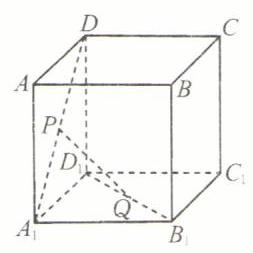
\includegraphics[width=0.15\textwidth]{bodyxb/src/bo_d20aucref24c73anc48g_140_392_1501_253_253_0.jpg}
    \end{center}
    \begin{jieda}
        连接 ${A}_{1}{C}_{1}$,与 ${B}_{1}{D}_{1}$ 的交点即点 $Q$. 在 $\bigtriangleup D{A}_{1}{C}_{1}$ 中, ${PQ}$ 是 $D{C}_{1}$ 边上的中位线,故 ${PQ}//D{C}_{1}$，而 $D{C}_{1}//A{B}_{1}$,故 ${PQ}//A{B}_{1}$,进而 ${PQ}//$ 平面 $A{A}_{1}{B}_{1}B$,证毕.
    \end{jieda}
    \item 如图,四棱锥 $P - {ABCD}$ 中, ${ABCD}$ 是平行四边形, $M$ 是 ${PC}$ 的中点.
    \begin{enumerate}
        \item 若 ${AB}$ 的中点为 $N$ ，求证: ${MN}//$ 平面 ${APD}$
        \item 在 ${DM}$ 上取一点 $G$ ，过 $G$ 和 ${AP}$ 作平面交平面 ${BDM}$ 于 ${GH}$ ， $H$ 在 ${BD}$ 上，证明: ${AP}//{GH}$
    \end{enumerate}
    \begin{center}
    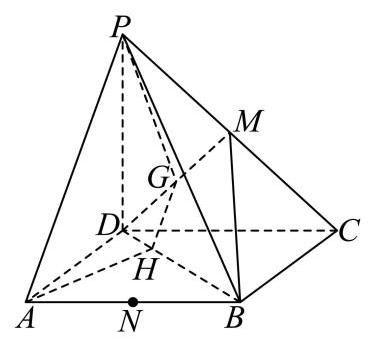
\includegraphics[width=0.15\textwidth]{bodyxb/src/0_1168_71_368_340_0.jpg}
    \end{center}
    \begin{jieda}
        \begin{enumerate}
            \item 证明如下:

            如图所示,取 ${PD}$ 的中点 $E$,连接 ${ME},{AE}$,

            因为 $M$ 为 ${PC}$ 的中点,可得 ${ME}//{CD}$ 且 ${ME} = \dfrac{1}{2}{CD}$,

            又因为 ${ABCD}$ 为平行四边形,可得 ${AB}//{CD}$ 且 ${AB} = {CD}$,

            所以 ${ME}//{AB}$ 且 ${ME} = \dfrac{1}{2}{AB}$,

            又因为 $N$ 为 ${AB}$ 的中点,可得 ${ME}//{AN}$ 且 ${ME} = {AN}$,

            所以四边形 ${ANME}$ 为平行四边形,所以 ${MN}//{AE}$,

            因为 ${MN} \not \subset$ 平面 ${PAD}$,且 ${AE} \subset$ 平面 ${PAD}$,所以 ${MN}//$ 平面 ${PAD}$.
            \item 证明如下:

            连接 ${AC}$ 与 ${BD}$ 交于点 $O$,且 $O$ 为 ${AC}$ 的中点,

            由点 $M$ 为 ${PC}$ 的中点,所以 ${AP}//{MO}$,

            因为 ${AP} \not \subset$ 平面 ${BDM}$,且 ${MO} \subset$ 平面 ${BDM}$,所以 ${AP}//$ 平面 ${BDM}$,

            又因为 ${AP} \subset$ 平面 ${AHGP}$,且平面 ${AHGP} \cap$ 平面 ${BDM} = {GH}$,所以 ${AP}//{GH}$.

            \begin{center}
            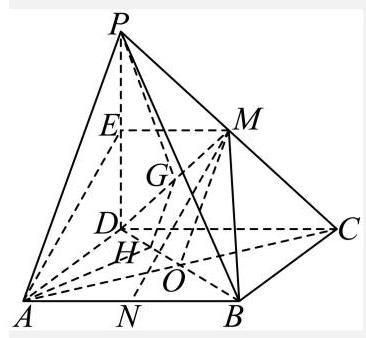
\includegraphics[width=0.15\textwidth]{bodyxb/src/0_91_1303_366_338_0.jpg}
            \end{center}
        \end{enumerate}
    \end{jieda}
    \item 如图，在$P - {ABCD}$ 中,侧棱 ${PD} \bot$ 长方形底面 ${ABCD}$, 且 ${PD} = {CD}$,过棱 ${PC}$ 的中点 $E$,作 ${EF} \bot  {PB}$ 交 ${PB}$ 于点 $F$,连接 ${DE},{DF},{BD},{BE}$. 证明: ${PB} \bot$ 平面 ${DEF}$.
    
    \begin{center}
    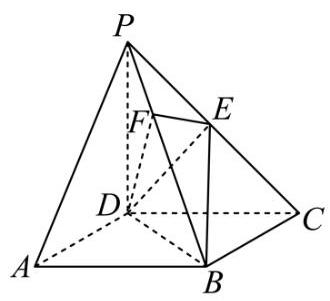
\includegraphics[width=0.15\textwidth]{bodyxb/src/bo_d4ofiljef24c73bbsnjg_0_240_718_330_301_0.jpg}
    \end{center}

    \begin{jieda}
        因为 ${PD} \bot$ 底面 ${ABCD}$, ${BC} \subset$ 底面 ${ABCD}$,所以 ${PD} \bot  {BC}$
        
        由底面 ${ABCD}$ 为长方形,有 ${BC} \bot  {CD}$,而 ${PD} \cap  {CD} = D,{PD},{CD} \subset$ 平面 ${PDC}$，所以 ${BC} \bot$ 平面 ${PCD}$,而 ${DE} \subset$ 平面 ${PCD}$，所以 ${BC} \bot  {DE}$
        
        又因为 ${PD} = {CD}$,点 $E$ 是 ${PC}$ 的中点,所以 ${DE} \bot  {PC}$
        
        而 ${PC} \cap  {BC} = C,{PC},{BC} \subset$ 面 ${PBC}$,所以 ${DE} \bot$ 平面 ${PBC}$
        
        而 ${PB} \subset$ 平面 ${PBC}$,所以 ${PB} \bot  {DE}$
        
        又 ${PB} \bot  {EF},{DE} \cap  {EF} = E,{DE},{EF} \subset$ 面 ${DEF}$,所以 ${PB} \bot$ 平面 ${DEF}$.
    \end{jieda}

        \item 如图,平面四边形 ${ABCD}$ 中, ${AB} = 8,{CD} = 3,{AD} = 5\sqrt{3},\angle {ADC} = {90}^{ \circ  },\angle {BAD} = {30}^{ \circ  }$ , 点 $E,F$ 满足 $\vv{AE} = \dfrac{2}{5}\vv{AD},\vv{AF} = \dfrac{1}{2}\vv{AB}$ ,将 $\bigtriangleup  {AEF}$ 沿 ${EF}$ 翻折至 $\bigtriangleup  {PEF}$. 证明: ${EF}\bot {PD}$

        \begin{center}
        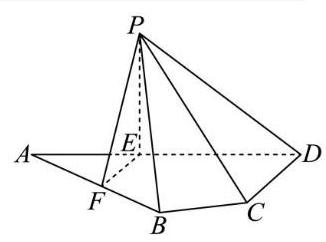
\includegraphics[width=0.15\textwidth]{bodyxb/src/10_1249_1364_326_242_0.jpg}
        \end{center}

        \begin{jieda}
            由 ${AB} = 8,{AD} = 5\sqrt{3},\vv{AE} = \dfrac{2}{5}\vv{AD},\vv{AF} = \dfrac{1}{2}\vv{AB}$ ，得 ${AE} = {2\sqrt{3}},{AF} = 4$ ，又 $\angle {BAD} = {30}^{ \circ  }$
                
            ${EF} = \sqrt{A{E}^{2} + A{F}^{2} - {2AE} \cdot  {AF}\cos \angle {BAD}} = \sqrt{{16} + {12} - 2 \cdot  4 \cdot  2\sqrt{3} \cdot  \dfrac{\sqrt{3}}{2}} = 2$

            所以 $A{E}^{2} + E{F}^{2} = A{F}^{2}$ ,则 ${AE} \bot  {EF}$ ,即 ${EF} \bot  {AD}$ ,

            所以 ${EF} \bot  {PE},{EF} \bot  {DE}$ ,又 ${PE} \cap  {DE} = E,{PE}\text{ 、 }{DE} \subset$ 平面 ${PDE}$ ,

            所以 ${EF} \bot$ 平面 ${PDE}$ ,又 ${PD} \subset$ 平面 ${PDE}$ ,故 ${EF} \bot  {PD}$
        \end{jieda}
        \item (2025$\cdot$宝山区一模$\cdot$17)如图所示，四棱锥 $P - {ABCD}$ 中，底面 ${ABCD}$ 为矩形， ${PA} = {PB} = {AD} =$ 3, ${AB} = 4$ ，且该四棱锥的体积为 $4\sqrt{5}$. 证明:平面 ${PAB} \bot$ 底面 ${ABCD}$
        \begin{center}
        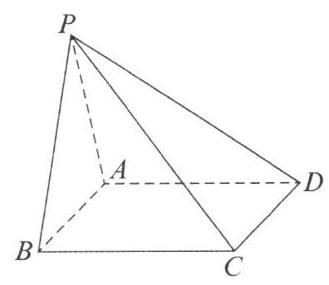
\includegraphics[width=0.15\textwidth]{bodyxb/src/156_1099_907_329_285_0.jpg}
        \end{center}
        \begin{jieda}
            证明:设该四棱锥的高为 $h$ ，则体积 $V = \dfrac{1}{3}S \times  h = \dfrac{1}{3} \times  3 \times  {4h} = 4\sqrt{5}$ ,从而 $h = \sqrt{5}$ ,等腰 $\bigtriangleup {PAB}$ 中,设边 ${AB}$ 的中点为 $E$ ,易知 ${PE} \bot  {AB}$ ,在 $\operatorname{Rt}\bigtriangleup {PAE}$ 中, ${PA} = 3,{AE} = 2$ ,所以 ${PE} = \sqrt{5}$ ,所以该四棱锥的高为 $h$ 即为 ${PE} = \sqrt{5}$ ,即 ${PE} \bot$ 底面 ${ABCD}$ ,又 ${PE} \subset$ 平面 ${PAB}$ ,所以平面 ${PAB} \bot$ 底面 ${ABCD}$ 
        \end{jieda}
\end{enumerate}
\subsection*{空间角与距离}
\begin{enumerate}
    \item (2024$\cdot$青浦区一模$\cdot$17)已知四棱锥 $P - {ABCD}$ ，底面 ${ABCD}$ 为正方形，边长为3， ${PD}\bot$ 平面 ${ABCD}$.
    \begin{enumerate}
        \item 求证: ${BC}\bot$ 平面 ${CDP}$
        \item 若直线 ${AD}$ 与 ${BP}$ 所成的角大小为 ${60}^{ \circ  }$ ，求 ${DP}$ 的长.
    \end{enumerate}
    \begin{center}
    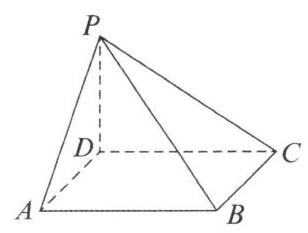
\includegraphics[width=0.15\textwidth]{bodyxb/src/166_1155_295_308_233_0.jpg}
    \end{center}
    \begin{jieda}
        \begin{enumerate}
            \item 因为 ${PD} \bot$ 平面 ${ABCD}$ ,所以 ${DP} \bot  {BC}$ ,又 ${BC} \bot  {DC}$ 且 ${DC} \cap  {DP} = D,{DC},{DP} \subset$ 平面 ${CDP}$ ,所以 ${BC} \bot$ 平面 ${CDP}$ ;

            \item 因为 ${BC} \bot$ 平面 ${CDP}$ ,所以 ${BC} \bot  {CP}$ ,所以 $\angle {CBP}$ 为锐角,又因为 ${AD}//{BC}$ ,所以 $\angle {CBP}$ 为直线 ${AD}$ 与 ${BP}$ 所成的角,所以 $\angle {CBP} = {60}^{ \circ  }$ ,所以 ${CP} = 3\sqrt{3}$ ,在 $\operatorname{Rt}\bigtriangleup {CDP}$ 中, ${CP} = 3\sqrt{3},{CD} = 3$ ,于是 ${DP} = 3\sqrt{2}$ .
        \end{enumerate}
    \end{jieda}
    \item (2025$\cdot$上海春季卷$\cdot$9)已知 $P$ 是一个圆锥的顶点， ${PA}$ 是母线， ${PA} = 2$， 圆锥的底面半径是 $1.B,C$ 分别在圆锥的底面上，则异面直线 ${PA}$ 与 ${BC}$ 所成角的最小值为\blkda[2]{$\dfrac{\pi }{3}$}.
    \begin{center}
    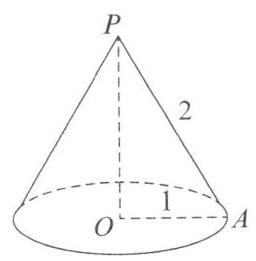
\includegraphics[width=0.15\textwidth]{bodyxb/src/159_1132_527_256_261_0.jpg}
    \end{center}
    \begin{jieda}
        线面角最小角定理: 直线 ${PA}$ 与底面上所有直线的夹角中,最小的角是 ${PA}$ 与底面的夹角,即 $\angle {PAO} = \dfrac{\pi }{3}$.
    \end{jieda}
    \item (2024$\cdot$静安区一模$\cdot$9)如图所示，在四棱锥 $P - {ABCD}$ 中， ${PA}\bot$ 平面 ${ABCD}$ ，底面 ${ABCD}$ 是矩形， $\left| {AP}\right|  = \left| {AB}\right|  = 2,\left| {AD}\right|  = 4,E$ 是 ${BC}$ 上的点， 直线 ${PB}$ 与平面 ${PDE}$ 所成的角是 $\arcsin \dfrac{\sqrt{3}}{6}$ ，则 ${BE}$ 的长为\blkda[2]{2}.

    \begin{center}
    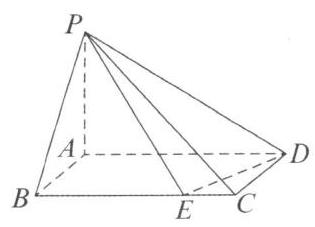
\includegraphics[width=0.15\textwidth]{bodyxb/src/160_1182_172_315_227_0.jpg}
    \end{center}
    \begin{jieda}
        由题意知在四棱锥中, ${PA} \bot$ 平面 ${ABCD}$ ,底面 ${ABCD}$ 是矩形，以 $A$ 为坐标原点，以射线 ${AB},{AD},{AP}$ 为 $x,y,z$ 轴的正半轴建立空间直角坐标系,则 $A(0$ , $0,0),B\left( {2,0,0}\right) ,P\left( {0,0,2}\right) ,D(0$ , $4,0)$ ,设 $E\left( {2,t,0}\right) \left( {0 \leq  t \leq  4}\right)$ ,则 $\vv{PB} = \left( {2,0, - 2}\right) ,\vv{PD} = (0$ , $4, - 2),\vv{PE} = \left( {2,t, - 2}\right)$ ,设平面 ${PDE}$ 的一个法向量为 $\vv{n} =  \left( {x,y,z}\right)$ ,则 $\left\{  \begin{array}{l} \vv{n} \cdot  \vv{PD} = 0 \\  \vv{n} \cdot  \vv{PE} = 0 \end{array}\right.$ ,即 $\left\{  \begin{array}{l} {4y} - {2z} = 0 \\  {2x} + {ty} - {2z} = 0 \end{array}\right.$ ,令 $y = 2$ ,则 $\vv{n} = \left( {4 - t,2,4}\right)$ ,设直线 ${PB}$ 与平面 ${PDE}$ 所成的角为 $\theta ,\theta  \in  \left\lbrack  {0,\dfrac{\pi }{2}}\right\rbrack$ ,直线 ${PB}$ 与平面 ${PDE}$ 所成的角是 $\arcsin \dfrac{\sqrt{3}}{6}$ ,则 $\sin \theta  = \dfrac{\sqrt{3}}{6}$ ,故 $\sin \theta  = \left| {\cos \langle \vv{n},\vv{PB}\rangle }\right|  = \dfrac{\left| \vv{n} \cdot  \vv{PB}\right| }{\left| \vv{n}\right| \left| \vv{PB}\right| } =  \dfrac{\left| 2t\right| }{2\sqrt{2} \cdot  \sqrt{{\left( 4 - t\right) }^{2} + {20}}} = \dfrac{\sqrt{3}}{6}$ ,解得 $t = 2$ ,故 ${BE} = 2$ .

        \begin{center}
        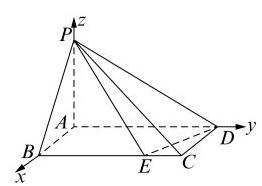
\includegraphics[width=0.15\textwidth]{bodyxb/src/118_607_1193_262_186_0.jpg}
        \end{center}
    \end{jieda}
    \item (2024$\cdot$松江区一模$\cdot$17)如图所示，在四棱锥 $P - {ABCD}$ 中， ${PA}\bot$ 底面 ${ABCD},{AB}\bot {AD}$ ，点 $E$ 在线段 ${AD}$ 上，且 ${CE}//{AB}$.
    \begin{enumerate}
        \item 求证: ${CE} \bot$ 平面 ${PAD}$
        \item 若四棱锥 $P - {ABCD}$ 的体积为 $\dfrac{5}{6}{AB} = 1,{AD} = 3,{CD} = \sqrt{2}$ ， $\angle {CDA} = {45}^{ \circ  }$ ,求二面角 $P - {CE} - A$ 的大小.
    \end{enumerate}
    \begin{center}
    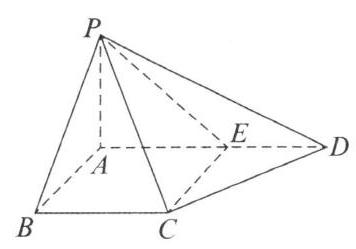
\includegraphics[width=0.15\textwidth]{bodyxb/src/165_1060_344_356_249_0.jpg}
    \end{center}
    \begin{jieda}
        \begin{enumerate}
            \item 如图所示， ${PA} \bot$ 底面 ${ABCD}$ ， ${CE} \subset$ 平面 ${ABCD} \Longrightarrow  {PA} \bot  {CE}$ ,又 ${AB} \bot {AD}$ ,且 ${CE}//{AB} \Longrightarrow  {CE} \bot  {AD},{PA} \cap  {AD} = A,{PA},{AD} \subset$ 平面 ${PAD}$ ,所以 ${CE} \bot$ 平面 ${PAD}$

            \item 由(1)得 ${CE} \bot$ 平面 ${PAD} \Longrightarrow  {CE} \bot  {PE},{CE} \bot  {AE}$ ，所以 $\angle {PEA}$ 为所求二面角 $P - {CE} - A$ 的平面角; 四棱锥的体积为 $\dfrac{5}{6}$ , ${V}_{P - {ABCD}} = \dfrac{1}{3}{Sh} = \dfrac{1}{3} \times  \dfrac{{BC} + {AD}}{2} \times  {AB} \times  {PA},{AB} = 1,{AD} =  3,{CD} = \sqrt{2},\angle {CDA} = {45}^{ \circ  }$ ,则 ${CE} = {AB} = 1,{ED} = {CE} = 1$ ,故 ${BC} = {AE} = 2$ ,代入体积公式可解得 ${PA} = h = 1,{PA} = 1$ ,$\tan \angle {PEA} = \dfrac{PA}{AE} = \dfrac{1}{2} \Longrightarrow  \angle {PEA} = \arctan \dfrac{1}{2}$ ,所以二面角 $P - {CE} - A$ 的平面角的大小为 $\arctan \dfrac{1}{2}$ .
        \end{enumerate}
    \end{jieda}
    \item (2024$\cdot$奉贤区一模$\cdot$5)在四面体 $P - {ABC}$ 中，若底面 ${ABC}$ 的一个法向量为 $\vv{n} = \left( {1,1,0}\right)$ ，且 $\vv{CP} = \left( {2,2, -1}\right)$ ，则顶点 $P$ 到底面 ${ABC}$ 的距离为\blkda[2]{$2\sqrt{2}$}.
    \begin{jieda}
        $d = \dfrac{\left| \vv{CP} \cdot  \vv{n}\right| }{\left| \vv{n}\right| } = \dfrac{1 \times  2 + 1 \times  2 + 0}{\sqrt{2}} = 2\sqrt{2}$.
    \end{jieda}
    \item 已知 $A\left( {3,1,0}\right)$ ， $B\left( {5,2,2}\right)$ ， $C\left( {4,1,2}\right)$ ，则点 $C$ 到直线 ${AB}$ 的距离为\blkda{1}.
    \begin{jieda}
        $\vv{AB} = \left( {2,1,2}\right) ,\left| \vv{AB}\right|  = \sqrt{{2}^{2} + {1}^{2} + {2}^{2}} = 3$ ，$\vv{AC} = \left( {1,0,2}\right)$，$\left| \vv{AC}\right|  = \sqrt{{1}^{2} + {2}^{2}} = \sqrt{5}$

        $\dfrac{\vv{AC} \cdot  \vv{AB}}{\left|\vv{AB}\right|} = 2$，故点 $C$ 到直线 ${AB}$ 的距离为: $d = \sqrt{{\left| \vv{AC}\right| }^{2} - {\left(\dfrac{\vv{AC} \cdot  \vv{AB}}{\left|\vv{AB}\right|}\right) }^{2}} = 1$.

    \end{jieda}
\end{enumerate}
\subsection*{平面问题的空间版本}
\begin{enumerate}
    \item (2025$\cdot$黄浦区一模$\cdot$8)在正四面体 ${ABCD}$ 中，点 $N$ 是 $\bigtriangleup  {ABC}$ 的中心，若 $\vv{DN} = \lambda \vv{DA} + \mu \vv{DB} +  \nu \vv{BC}\left( {\lambda ,\mu ,\nu  \in  \mathbf{R}}\right)$ ，则 $\lambda  + \mu  + \nu  =$ \blkda[2]{$\dfrac{4}{3}$}.
    \begin{jieda}
        $\vv{DN} = \lambda \vv{DA} + \mu \vv{DB} +  \nu (\vv{DC} - \vv{DB}) = \lambda \vv{DA} + (\mu - \nu) \vv{DB} + \nu \vv{DC} = \dfrac{1}{3} \vv{DA} + \dfrac{1}{3} \vv{DB} + \dfrac{1}{3} \vv{DC}$

        故$\left\{\begin{array}{l}
            \lambda = \dfrac{1}{3} \\
            \mu = \dfrac{2}{3} \\
            \nu = \dfrac{1}{3}
        \end{array}\right.$
    \end{jieda}
    \item (2025$\cdot$普陀区一模$\cdot$9)设 $\lambda  \in  \mathbf{R}$ ，在如图所示的平行六面体 ${ABCD} - {A}_{1}{B}_{1}{C}_{1}{D}_{1}$ 中， $\angle {A}_{1}{AB} =  \angle {A}_{1}{AD} = \angle {BAD} = \dfrac{\pi }{3},A{A}_{1} = 2,{AB} = {AD} = 1$ ,点 $M$ 是棱 ${C}_{1}{D}_{1}$ 的中点， $\vv{{A}_{1}N} = \lambda \vv{{A}_{1}{D}_{1}}$ ，若 $\vv{AM} \cdot  \vv{CN} = 2$ ,则 $\lambda$ 的值为\blkda[2]{$\dfrac{1}{3}$}.

    \begin{center}
    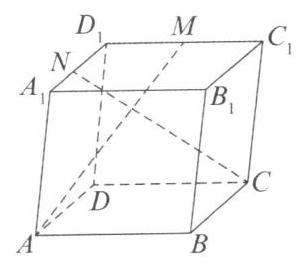
\includegraphics[width=0.15\textwidth]{bodyxb/src/159_1017_1734_298_264_0.jpg}
    \end{center}


    \begin{jieda}
        设 $\vv{AB} = \vv{a},\vv{AD} = \vv{b},\vv{A{A}_{1}} = \vv{c}$ , 由 $\angle {A}_{1}{AB} = \angle {A}_{1}{AD} = \angle {BAD} = \dfrac{\pi }{3}$ , $A{A}_{1} = 2,{AB} = {AD} = 1$ ,可得 $\left| \vv{a}\right|  = \left| \vv{b}\right|  = 1,\left| \vv{c}\right|  = 2,\vv{a} \cdot  \vv{b} = \dfrac{1}{2},\vv{a} \cdot  \vv{c} = \vv{b} \cdot  \vv{c}  = 1$ ,因为点 $M$ 是棱 ${C}_{1}{D}_{1}$ 的中点, $\vv{{A}_{1}N} = \lambda \vv{{A}_{1}{D}_{1}}$ ,所以 $\vv{AM}$ . $\vv{CN} = \left( {\vv{A{A}_{1}} + \vv{{A}_{1}{D}_{1}} + \vv{{D}_{1}M}}\right)  \cdot  \left( {\vv{AN} - \vv{AC}}\right)  = \left( {\vv{c} + \vv{b} + \dfrac{1}{2}\vv{a}}\right)$ . $\left\lbrack  {\vv{c} + \lambda \vv{b} - \left( {\vv{a} + \vv{b}}\right) }\right\rbrack   = \left( {\dfrac{1}{2}\vv{a} + \vv{b} + \vv{c}}\right)  \cdot  \left\lbrack  {-\vv{a} + \left( {\lambda  - 1}\right) \vv{b} + \vv{c}}\right\rbrack  =  - \dfrac{1}{2}{\vv{a}}^{2} + \left( {\lambda  - 1}\right) {\vv{b}}^{2} + {\vv{c}}^{2} + \dfrac{\lambda  - 3}{2}\vv{a} \cdot  \vv{b} - \dfrac{1}{2}\vv{a} \cdot  \vv{c} + \lambda \vv{b} \cdot  \vv{c} =  - \dfrac{1}{2} + \lambda  - 1 + 4 + \dfrac{\lambda  - 3}{4} - \dfrac{1}{2} + \lambda  = \dfrac{9\lambda }{4} + \dfrac{5}{4} = 2$ ,解得 $\lambda  = \dfrac{1}{3}$.
        \begin{center}
            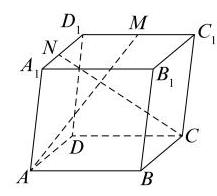
\includegraphics[width=0.15\textwidth]{bodyxb/src/118_647_540_217_196_0.jpg}
        \end{center}
    \end{jieda}
    \item (2025$\cdot$浦东新区二模$\cdot$11)已知 $\vv{a}$ 、 $\vv{b}$ 、 $\vv{c}$ 为空间中三个单位向量，且 $\vv{a} \cdot  \vv{b} = \vv{b} \cdot  \vv{c} = \vv{c} \cdot  \vv{a} = 0$ ，若向量 $\vv{p}$ 满足 $\left| {\vv{p} - 2\vv{a}}\right|  = \dfrac{3}{2},\left| {\vv{p} - 2\vv{b}}\right|  = \dfrac{3}{2}$ ，则向量 $\vv{p}$ 与向量 $\vv{c}$ 夹角的最小值为\blkda[2]{$\arccos \dfrac{\sqrt{2}}{4}$}. (用反三角表示)
    \begin{jieda}
        可设 $\vv{a} = \left( {1,0,0}\right) ,\vv{b} = \left( {0,1,0}\right) ,\vv{c} = \left( {0,0,1}\right)$ ,设 $\vv{p} =  \left( {x,y,z}\right)$ ,则 $\vv{p} - 2\vv{a} = \left( {x - 2,y,z}\right) ,\vv{p} - 2\vv{b} = \left( {x,y - 2,z}\right)$ , 所以 $\left\{  \begin{array}{l} {\left( x - 2\right) }^{2} + {y}^{2} + {z}^{2} = \dfrac{9}{4} \\  {x}^{2} + {\left( y - 2\right) }^{2} + {z}^{2} = \dfrac{9}{4} \end{array}\right.$ ,两式相减可得: $x = y$ ,再代入第一个式子,可得: $2{x}^{2} + {z}^{2} = {4x} - \dfrac{7}{4}$ ,设向量 $\vv{p}$ 与向量 $\vv{c}$ 夹角为 $\theta$ ,则 $\cos \theta  = \dfrac{z}{\sqrt{{x}^{2} + {y}^{2} + {z}^{2}}} = \dfrac{\sqrt{{4x} - \dfrac{7}{4} - 2{x}^{2}}}{\sqrt{{4x} - \dfrac{7}{4}}} =  \sqrt{1 - \dfrac{2{x}^{2}}{{4x} - \dfrac{7}{4}}} = \sqrt{1 - \dfrac{2}{\dfrac{4}{x} - \dfrac{7}{4{x}^{2}}}}$ ,易知对于 $y =  - \dfrac{7}{4{x}^{2}} + \dfrac{4}{x}$ 当 $\dfrac{1}{x} = \dfrac{8}{7}$ 即 $x = \dfrac{7}{8}$ 取得最大值 $\dfrac{16}{7}$ ,此时 $\sqrt{1 - \dfrac{2}{\dfrac{4}{x} - \dfrac{7}{4{x}^{2}}}}$ 取得最大值 $\dfrac{\sqrt{2}}{4}$ ，即 $\cos \theta$ 的最大值为 $\dfrac{\sqrt{2}}{4}$ ， $x = \dfrac{7}{8}$ 时取得，再由余弦函数的单调性可知 $\theta$ 的最小值为 $\arccos \dfrac{\sqrt{2}}{4}$.
    \end{jieda}
    \item (2025$\cdot$普陀区二模$\cdot$11)在棱长为 4 的正方体 ${ABCD} - {A}_{1}{B}_{1}{C}_{1}{D}_{1}$ 中， $\vv{AN} = 2\vv{AM} = \dfrac{1}{2}\vv{A{C}_{1}}$ ，若一动点 $G$ 满足 $\left| \vv{GN}\right|  = \sqrt{2}\left| \vv{GM}\right|$ ，则三棱锥 $G - {A}_{1}{B}_{1}{D}_{1}$ 体积的最大值为\blkda[2]{$\dfrac{{32} + 8\sqrt{6}}{3}$}.
    \begin{jieda}
        如图,以 $A$ 为坐标原点建立空间直角坐标系,则有 $A\left( {0,0,0}\right) ,{C}_{1}\left( {4,4,4}\right)$ . 又 $\vv{AN} = 2\vv{AM} = \dfrac{1}{2}\vv{A{C}_{1}}$ ,所以 $M(1,1,1),N\left( {2,2,2}\right)$.
        
        设 $G\left( {x,y,z}\right)$ ,则 $\vv{GN} = (2 - x,2 - y,2 -  z),\vv{GM} = \left( {1 - x,1 - y,1 - z}\right)$ . 因为 $\left| \vv{GN}\right|  = \sqrt{2}\left| \vv{GM}\right|$ ,代入可得 ${\left( 2 - x\right) }^{2} + {\left( 2 - y\right) }^{2} + {\left( 2 - z\right) }^{2} = 2\left\lbrack {\left( 1 - x\right) }^{2} + {\left( 1 - y\right) }^{2} +{\left( 1 - z\right) }^{2}\right\rbrack$ ,整理可得 ${x}^{2} + {y}^{2} + {z}^{2} = 6$ ,即 $G$ 在以点 $A$ 为球心， $r = \sqrt{6}$ 为半径的球上. 又 ${{Rt}}\bigtriangleup {A}_{1}{B}_{1}{D}_{1}$ 的面积为 ${S}_{\bigtriangleup {A}_{1}{B}_{1}{D}_{1}} = \dfrac{1}{2} \times  4 \times  4 = 8$ ，平面 ${ABCD}$ 到平面 ${A}_{1}{B}_{1}{C}_{1}{D}_{1}$ 的距离为 4,所以 $G$ 到平面 ${A}_{1}{B}_{1}{D}_{1}$ 的最大距离为 ${d}_{\max } = 4 + r = 4 + \sqrt{6}$ . 体积最大值为 $V = \dfrac{1}{3} \times  {S}_{\bigtriangleup {A}_{1}{B}_{1}{D}_{1}} \times  {d}_{\max } = \dfrac{1}{3} \times  8 \times  \left( {4 + \sqrt{6}}\right)  = \dfrac{{32} + 8\sqrt{6}}{3}.$
        \begin{center}
        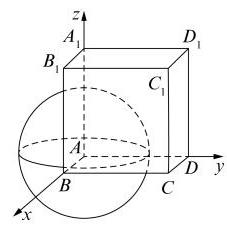
\includegraphics[width=0.15\textwidth]{bodyxb/src/111_1301_1944_227_225_0.jpg}
        \end{center}
    \end{jieda}
\end{enumerate}
\subsection*{最短路径}
\begin{enumerate}
    \item 已知在圆锥 ${SO}$ 中,底面圆 $O$ 的直径 ${AB} = 2$ ,圆锥 ${SO}$ 的体积为 $\dfrac{2\sqrt{2}}{3}\pi$ ,点 $M$ 在母线 ${SB}$ 上, 且 $\vv{SM} = \dfrac{1}{3}\vv{SB}$ ，一只蚂蚁若从 $A$ 点出发，沿圆锥侧面爬行到达 $M$ 点，则它爬行的最短距离为\blkda{$\sqrt{7}$}.
    \begin{center}
    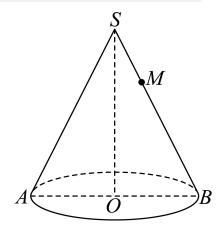
\includegraphics[width=0.15\textwidth]{bodyxb/src/0_1352_1376_219_227_0.jpg}
    \end{center}
    \begin{jieda}
        设圆锥 ${SO}$ 的母线长为 $l$ ,底面的半径为 $r = 1$ ,
        
        圆锥 ${SO}$ 的体积为 $\dfrac{1}{3}\pi  \times  {1}^{2} \times  {SO} = \dfrac{2\sqrt{2}}{3}\pi$ ,解得 ${OS} = 2\sqrt{2}$ .
        
        由勾股定理,可得母线 $l = \sqrt{{1}^{2} + {\left( 2\sqrt{2}\right) }^{2}} = 3$ ,
        
        \begin{center}
        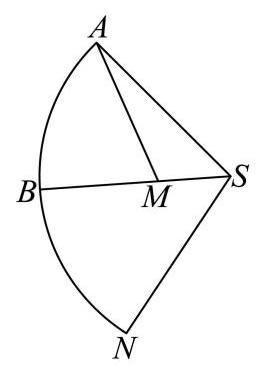
\includegraphics[width=0.15\textwidth]{bodyxb/src/0_1280_1762_256_368_0.jpg}
        \end{center}
        
        
        如图,圆锥的侧面展开图为扇形 ${SAN}$ ,在该扇形展开图中的计算如下,
        
        因为扇形 ${SAN}$ 的弧长为 ${2\pi r} = {2\pi }$ ，所以扇形 ${SAN}$ 的圆心角 $\angle {ASN} = \dfrac{2\pi }{l} = \dfrac{2\pi }{3}$ ，则 $\angle {ASM} = \dfrac{\pi }{3}$ ， 在 $\bigtriangleup {SAM}$ 中,由余弦定理可得 $A{M}^{2} = S{A}^{2} + S{M}^{2} - {2SA} \cdot  {SM}\cos \angle {ASM} = 9 + 1 - 3 = 7$ ,所以 ${AM} = \sqrt{7}$ ,因为 ${SA} + {SM} = 4 > \sqrt{7}$ ,所以蚂蚁爬行的最短距离为 ${AM}$ 的长度,即蚂蚁爬行的最短距离为 $\sqrt{7}$ .
    \end{jieda}
    \item 暑假将临，大学生小明同学准备利用假期探访名胜古迹. 已知某座山高耸入云，整体呈圆锥形，其半山腰(母线的中点) 有一座古寺，与上山入口在同一条母线上，入口和古寺通过一条盘山步道相连，且当时为了节省资金，该条盘山步道是按 “到达古寺的路程最短” 修建的. 如图, 已知该座山的底面半径 $R = 2\left( {{km}}\right)$ ，高 $h = 4\sqrt{2}\left( {{km}}\right)$ ，则盘山步道的长度为\blkda{$3\sqrt{7}km$}，其中上山(到山顶的直线距离减小)和下山(到山顶的直线距离增大) 路段的长度之比为\blkda{$5:2$}.
    
    \begin{center}
    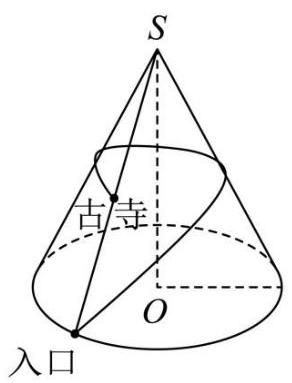
\includegraphics[width=0.15\textwidth]{bodyxb/src/bo_d5b4icbef24c73bio840_1_232_1116_292_383_0.jpg}
    \end{center}

    \begin{jieda}
        设入口为点 ${A}$ ,古寺位置为 $B$ ,则由题意, $B$ 为母线 ${SA}$ 的中点,
        由底面圆半径为 $2{{km}}$ ,山高为 $4\sqrt{2}{{km}}$ ,则母线 ${SA} = \sqrt{{2}^{2} + {\left( 4\sqrt{2}\right) }^{2}} = 6$ ,
        底面圆周长 ${2\pi r} = {4\pi }$ ,所以展开图的圆心角 $a = \dfrac{4\pi }{6} = \dfrac{2\pi }{3}$ ,
        作圆锥侧面展开图, 如图,
        \begin{center}
            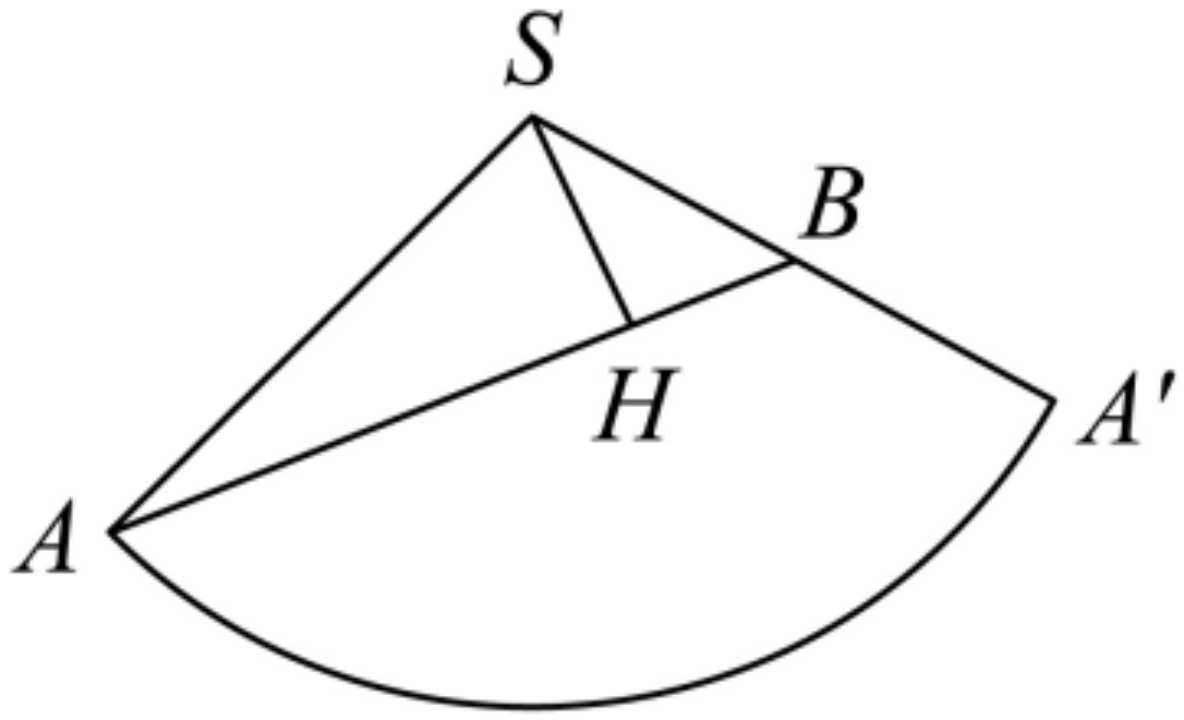
\includegraphics[width=0.2\linewidth]{bodyxb//src/zhuiti5.png}
        \end{center}
        由余弦定理可得 ${AB} = \sqrt{A{S}^{2} + S{B}^{2} - {2AS} \cdot  {SB}\cos \dfrac{2\pi }{3}} = \sqrt{{6}^{2} + {3}^{2} - 2 \times  6 \times  3 \times  \left( {-\dfrac{1}{2}}\right) } = 3\sqrt{7}$ ,
        由点 ${S}$ 向 ${AB}$ 引垂线,垂足为点 $H$ ,此时 ${SH}$ 为点 ${S}$ 和线段 ${AB}$ 上的点连线的最小值,
        即点 $H$ 为公路的最高点, ${AH}$ 段为上坡路, ${HB}$ 段为下坡路段,
        由 $\dfrac{1}{2}{SA} \cdot  {SB} \cdot  \sin \dfrac{2\pi }{3} = \dfrac{1}{2}{AB} \cdot  {SH}$ 可得, ${SH} = \dfrac{3\sqrt{21}}{7}$ ,
        所以 ${AH} = \sqrt{S{A}^{2} - S{H}^{2}} = \sqrt{{36} - \dfrac{27}{7}} = \dfrac{{15}\sqrt{7}}{7},{HB} = {AB} - {AH} = \dfrac{6\sqrt{7}}{7}$，所以上山和下山路段的长度之比为 $5 : 2$ .
    \end{jieda}
\end{enumerate}
\subsection*{动点问题}
\begin{enumerate}
    \item 如图,已知点 $P$ 在平行四边形 ${ABCD}$ 所在平面外, $E$ 为线段 ${AD}$ 上靠近 $A$ 的三等分点, $F$ 为线段 ${PC}$ 上一点,当 ${PA}//$ 平面 ${EBF}$ 时, $\dfrac{PC}{PF} =$ \blkda{4}
    \begin{center}
    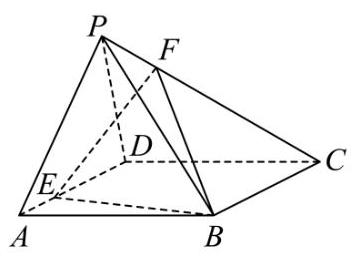
\includegraphics[width=0.15\textwidth]{bodyxb/src/bo_d4lnl5ref24c739do320_3_241_1515_352_258_0.jpg}
    \end{center}
    \begin{jieda}
        如图,连结 ${AC}$,交 ${BE}$ 于点 $M$,连结 ${FM}$
        
        \begin{center}
        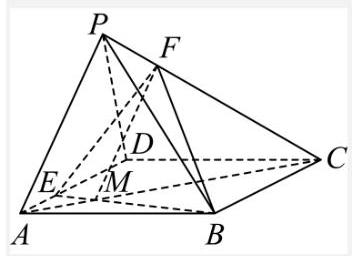
\includegraphics[width=0.15\textwidth]{bodyxb/src/bo_d4lnl5ref24c739do320_4_240_477_352_256_0.jpg}
        \end{center}

        因为 ${PA}//$ 平面 ${EBF}$,且 ${PA} \subset$ 平面 ${PAC}$,平面 ${PAC} \cap$ 平面 ${BEF} = {FM}$，所以$PA//FM$
        
        因为 ${AE}//{BC}$ ，且 ${AE} : {BC} = 1 : 3$ ，所以 ${AM} : {MC} = 1 : 3$ ，即 ${AM} : {AC} = 1 : 4$，所以 $\dfrac{PC}{PF} = 4$.
    \end{jieda}
    \item 在棱长为 2 的正方体 ${ABCD} - {A}_{1}{B}_{1}{C}_{1}{D}_{1}$ 中，点 $E,F$ 分别是棱 ${BC},{C{C}_{1}}$ 的中点，动点 $P$ 是侧面 ${BC}{C}_{1}{B}_{1}$ 内一点，若 ${A}_{1}P//$ 平面 ${AEF}$ ，则点 $P$ 的轨迹长度为\blkda{$\sqrt{2}$}.

    \begin{jieda}
        如下图所示,分别取棱 $B{B}_{1},{B}_{1}{C}_{1}$ 的中点 $M\text{ 、 }N$,连接 ${MN},B{C}_{1}$
        
        \begin{center}
        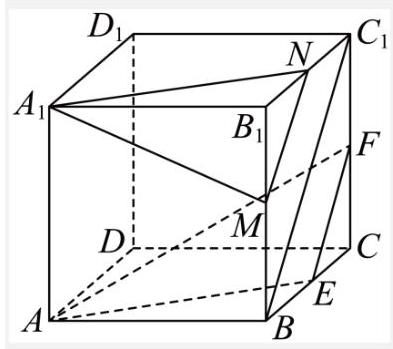
\includegraphics[width=0.15\textwidth]{bodyxb/src/bo_d50clvjef24c73bfi5dg_3_241_1779_393_349_0.jpg}
        \end{center}

        $MN // EF$，$A_1N // AE$，故平面$A_1MN // $平面$AEF$，故$P$的轨迹为$MN$，因此其长度为$\sqrt{2}$.
    \end{jieda}
        \item 已知四棱柱 ${ABCD} - {A}_{1}{B}_{1}{C}_{1}{D}_{1}$ 的底面为菱形， $A{A}_{1} \bot$ 底面 ${ABCD},A{A}_{1} = 6,{AB} = 6$ ， $\angle {BCD} = {60}^{ \circ  }$,点 $M$ 是线段 ${BC}$ 上靠近 $C$ 的三等分点,点 $N$ 在四棱柱 ${ABCD} - {A}_{1}{B}_{1}{C}_{1}{D}_{1}$ 的表面上移动，且 ${MN}\bot {A}_{1}C$ ，则动点 $N$ 的轨迹长度为\blkda{$2 + 2\sqrt{13}$}.

    \begin{jieda}
        如图所示
            
        \begin{center}
        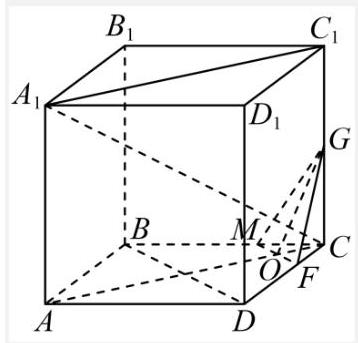
\includegraphics[width=0.15\textwidth]{bodyxb/src/bo_d50clvjef24c73bfi5dg_8_241_1196_358_343_0.jpg}
        \end{center}
    
        取$CD$上靠近$C$的三等分点，则$MF \bot AC$，取$CC_1$中点$G$，故平面$MFG \bot $平面$ACC_1A_1$，因为$AC \bot OG$，所以$AC \bot$平面$GMF$，故$N$的轨迹为$\triangle MFG$，则动点 $N$ 的轨迹长度为 ${MF} + {MG} + {FG} = 2 + 2\sqrt{13}$.
    \end{jieda}
\end{enumerate}